\documentclass[border=3pt,tikz]{standalone}
\usepackage[utf8]{vietnam}
\usetikzlibrary{calc,angles,intersections,shapes.geometric,arrows,decorations.markings,arrows.meta,patterns.meta,patterns}
\usepackage{tikz-3dplot,pgfplots}
\pgfplotsset{compat=1.15}
\usepgfplotslibrary{polar}
\usepackage{amsmath}
\begin{document}
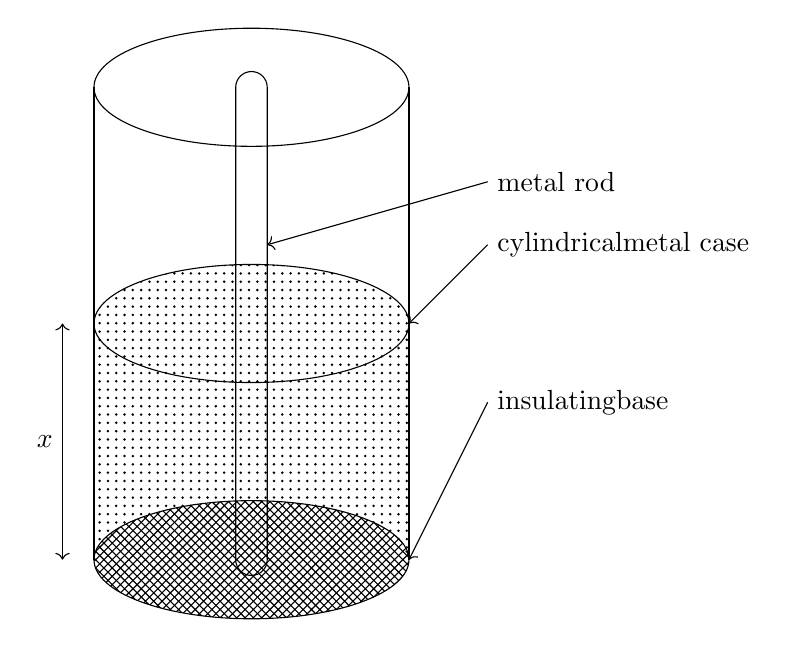
\begin{tikzpicture}
	\def\a{2}
	\def\b{0.75}
	\def\h{6}
	\fill[pattern=crosshatch] (0,0) ellipse ({\a} and {\b});
	\fill[pattern=dots] (\a,0) arc [ start angle=0, end angle=180, x radius=\a,y radius=\b] -- (-\a,\h/2) arc [ start angle=180, end angle=0, x radius=\a,y radius=\b] --cycle;
	\draw (0,0) ellipse ({\a} and {\b});
	\draw (0,\h/2) ellipse ({\a} and {\b});
	\draw (0,\h) ellipse ({\a} and {\b});
	\draw (\a,0)--(\a,\h) (-\a,0) -- (-\a,\h);
	\draw (\a/10,0)--(\a/10,\h) arc(0:180:\a/10) --(-\a/10,0) arc(180:360:\a/10);
	\draw[<->] (-1.2*\a,0) --(-1.2*\a,\h/2) node[midway, left]{$x$};
	\draw[->] (3*\a/2,4*\h/5) node[right]{metal rod}--(\a/10,2*\h/3);
	\draw[->] (3*\a/2,2*\h/3) node[right]{cylindrical \\ metal case}--(\a,\h/2);
	\draw[->] (3*\a/2,\h/3) node[right]{insulating\\ base}--(\a,0);
\end{tikzpicture}
\end{document}